\section{Use Case Model for METRICSTICS\\}
\begin{figure}[htp]
    \centering
    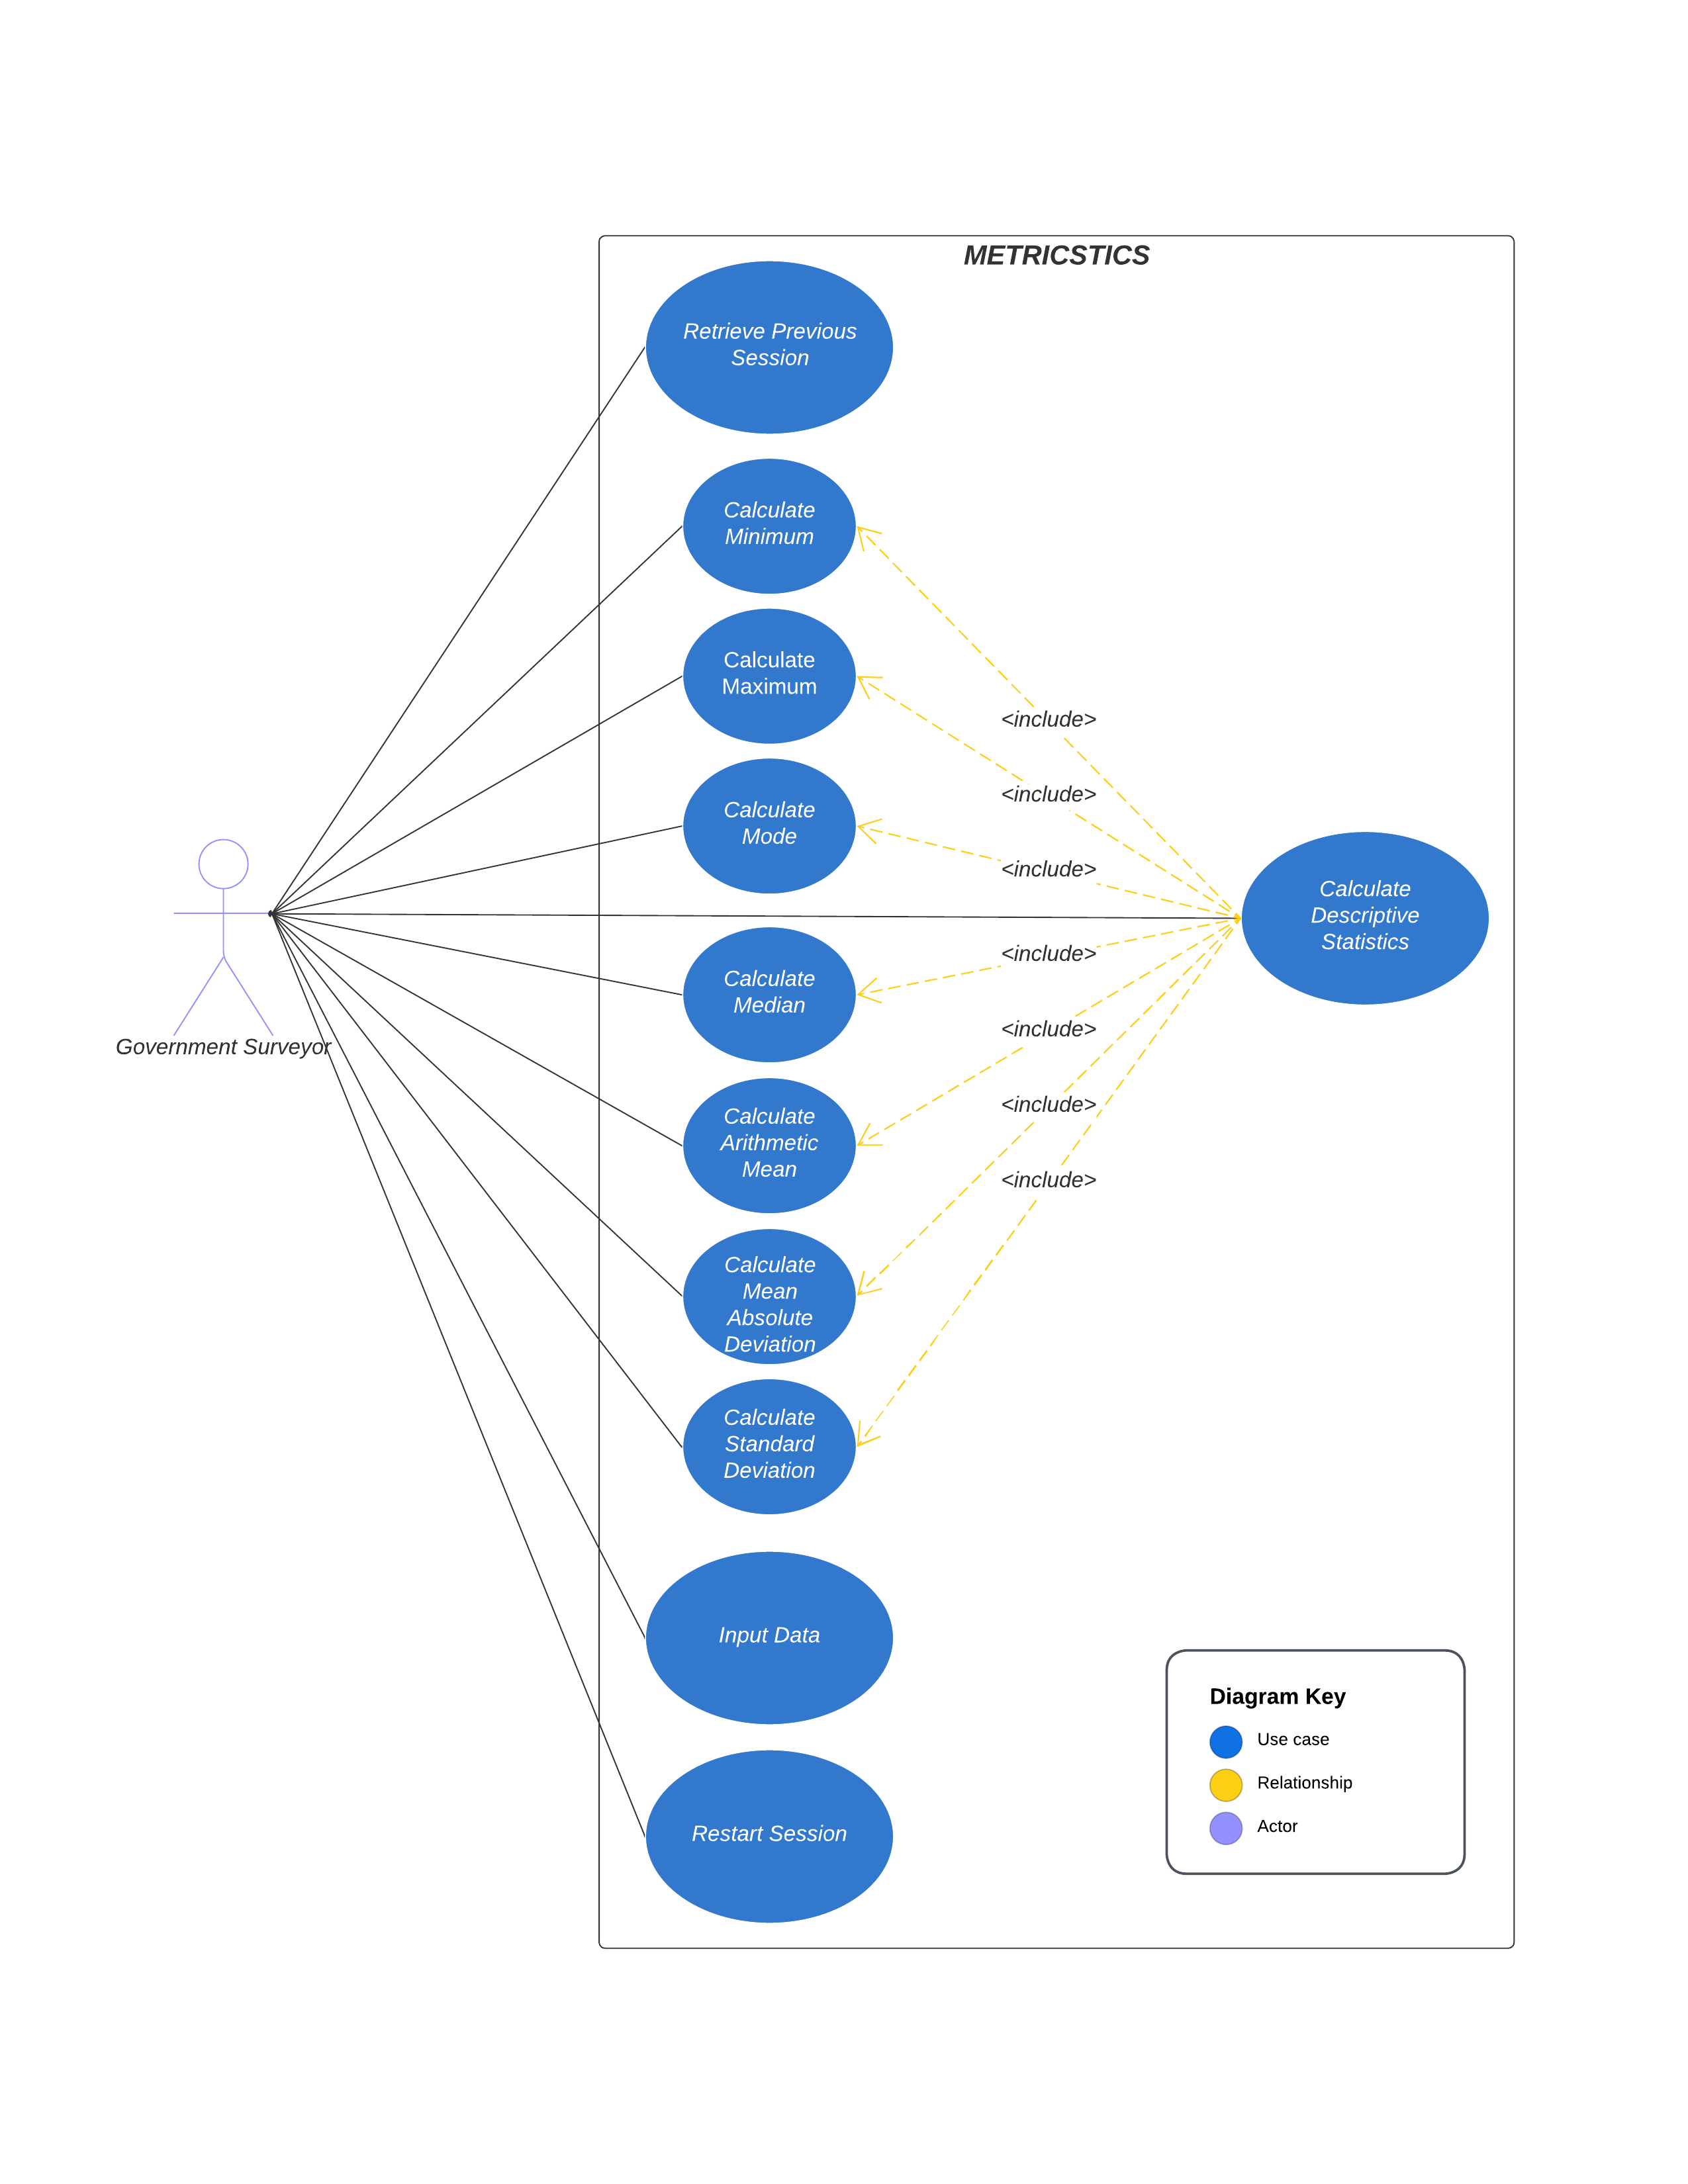
\includegraphics[width=12cm,height=10cm]{userModelingGraph.png}
    \renewcommand{\thefigure}{\arabic{figure}}
    \caption{A user modeling graph}
    \label{fig:figure1}
\end{figure}

\section{Actors}
\begin{itemize}
    \item \textbf{User:} Government Surveyor \\The primary user of the Metricstics system, representing a surveyor working for the government. This surveyor's responsibilities may include collecting and analyzing data from surveys, censuses, and various government-related studies.
    % \item \textbf{Data Source:} An external source providing data to METRICSTICS for analysis, which can be real or artificially generated.
    % \item \textbf{Administrator:} Responsible for maintaining and updating METRICSTICS, ensuring its security and compliance with regulations.
\end{itemize}
\hfill \break



\section{Use cases}


%table one

\begin{table}[h]
\subsection*{Use case 1}
\addcontentsline{toc}{subsection}{\protect\numberline{}Use case 1}
\begin{tabular}{ | p{4cm} | p{10cm} | }
 \hline
 \multicolumn{2}{|c|}{System: Metricstics} \\
 \hline
 Identifier: & UC-01 (Input Data) \\
 \hline
 Author(s): & Anirudh Boddu, anirudh.boddu@mail.concordia.ca  \\
 \hline
 Version: & 1.0	\\
 \hline
 Priority: & High	\\
 \hline
 Name: & Input Data	 \\
 \hline
 Pre-Condition(s):  & {1. The system is running and accessible.\newline
 2. The government surveyor has initiated a session.}\\
 \hline
 Post-Condition(s):  & {1. Data has been successfully entered and saved by the system.}\\
 \hline
 Trigger: & Government surveyor initiates data input. \\
 \hline
 Normal Flow:  & {1. Government surveyor selects "Input Data" option.\newline 2. Surveyor chooses to upload a CSV file or manually enter data.\newline 3. Surveyor provides data as per the selected method.\newline 4. System validates and accepts the data.\newline 5. Use case ends.}\\
 \hline
 Exceptional Flow(s):  & {1. Surveyor cancels data input.\newline 2. Data format is incorrect or incomplete.\newline 3. System encounters an error.}\\
 \hline
 Related Actor(s): & Government Surveyor\\
 \hline
 Related Use Case(s): & Calculate Descriptive Statistics (All-in-One), Calculate Mean, Calculate Minimum, Calculate Maximum, Calculate Median, Calculate Mode, Calculate Mean Absolute Deviation, Calculate Standard Deviation.\\
 \hline
 \end{tabular}
\renewcommand{\thetable}{\arabic{table}}
\caption{Use Case 1: Input Data}
\label{tab:table1}
\end{table}

%table two

\begin{table}[h]
\subsection*{Use case 2}
\addcontentsline{toc}{subsection}{\protect\numberline{}Use case 2}
\begin{tabular}{ | p{4cm} | p{10cm} | }
 \hline
 \multicolumn{2}{|c|}{System: Metricstics} \\
 \hline
 Identifier: & UC-02 (Calculate Descriptive Statistics (All-in-One)) \\
 \hline
 Author(s): & Anirudh Boddu, anirudh.boddu@mail.concordia.ca  \\
 \hline
 Version: & 1.0	\\
 \hline
 Priority: & High	\\
 \hline
 Name: & Calculate Descriptive Statistics (All-in-One)	 \\
 \hline
 Pre-Condition(s):  & {1. Data input has been completed (Use Case 1).\newline 2. The system has received valid data for analysis.}\\
 \hline
 Post-Condition(s):  & {1. Descriptive statistics (minimum, maximum, mean, median, mode, MAD, and standard deviation) have been calculated and displayed to the user.}\\
 \hline
 Trigger: & Government surveyor selects "Calculate Descriptive Statistics" option. \\
 \hline
 Normal Flow:  & {1. Government surveyor selects "Calculate Descriptive Statistics" option.\newline 2. System processes the input data.\newline 3. System calculates minimum, maximum, mean, median, mode, MAD, and standard deviation.\newline 4. System displays the results to the user.\newline 5. Use case ends.}\\
 \hline
 Exceptional Flow(s):  & {1. Data input is missing or invalid.\newline 2. System encounters an error during calculations.}\\
 \hline
 Related Actor(s): & Government Surveyor\\
 \hline
 Related Use Case(s): & Calculate Minimum, Calculate Maximum, Calculate Mean, Calculate Median, Calculate Mode, Calculate Mean Absolute Deviation, Calculate Standard Deviation.\\
 \hline
 \end{tabular}
\renewcommand{\thetable}{\arabic{table}}
\caption{Use Case 2: Calculate Descriptive Statistics (All-in-One)}
\label{tab:table1}
\end{table}

%table three

\begin{table}[h]
\subsection*{Use case 3}
\addcontentsline{toc}{subsection}{\protect\numberline{}Use case 3}
\begin{tabular}{ | p{4cm} | p{10cm} | }
 \hline
 \multicolumn{2}{|c|}{System: Metricstics} \\
 \hline
 Identifier: & UC-03 (Calculate Minimum) \\
 \hline
 Author(s): & Ayushi Chaudhary, ayushivihan@gmail.com    \\
 \hline
 Version: & 1.0	\\
 \hline
 Priority: & High	\\
 \hline
 Name: & Calculate Minimum  \\
 \hline
 Pre-Condition(s):  & {1. The METRICSTICS system is running and accessible. \newline 2. A government surveyor has initiated a session and provided data.  }\\
 \hline
 Post-Condition(s):  & {1. The minimum value from the dataset has been successfully calculated. }\\
 \hline
 Trigger: & Government surveyor selects the "Calculate Minimum" option. \\
 \hline
 Normal Flow:  & {1. Government surveyor selects the "Calculate Minimum" option from the available choices. \newline 2. METRICSTICS processes the data from the dataset. \newline 3. METRICSTICS calculates the minimum value. \newline 4. The minimum value is displayed to the government surveyor. \newline 5. Use case ends.}\\
 \hline
 Exceptional Flow(s):  & {1. No Data Available: \newline
   - If there is no data available in the dataset, METRICSTICS displays an error message indicating the unavailability of data for calculation.\newline
   - Use case ends.\newline
   2. Error in Calculation: \newline
   - If an unexpected error occurs during the calculation process (e.g., data format error), METRICSTICS displays an error message. \newline
   - Government surveyor may retry the operation with corrected data. \newline
   - Use case ends.}\\
 \hline
 Related Actor(s): & Government Surveyor\\
 \hline
 Related Use Case(s): & Input Data, Calculate Maximum, Calculate Mean, Calculate Median, Calculate Mode, Calculate Mean Absolute Deviation, Calculate Standard Deviation.\\
 \hline
 \end{tabular}
\renewcommand{\thetable}{\arabic{table}}
\caption{Use Case 3: Calculate Minimum}
\label{tab:table1}
\end{table}

%table four
\begin{table}[h]
\subsection*{Use case 4}
\addcontentsline{toc}{subsection}{\protect\numberline{}Use case 4}
\begin{tabular}{ | p{4cm} | p{10cm} | }
 \hline
 \multicolumn{2}{|c|}{System: Metricstics} \\
 \hline
 Identifier: & UC-04 (Calculate Maximum)  \\
 \hline
 Author(s): & Ayushi Chaudhary, ayushivihan@gmail.com    \\
 \hline
 Version: & 1.0	\\
 \hline
 Priority: & High	\\
 \hline
 Name: & Calculate Maximum \\
 \hline
 Pre-Condition(s):  & {1. The METRICSTICS system is running and accessible. \newline 2. A government surveyor has initiated a session and provided data.  }\\
 \hline
 Post-Condition(s):  & {1. The maximum value from the dataset has been successfully calculated.  }\\
 \hline
 Trigger: & Government surveyor selects the "Calculate Maximum" option.  \\
 \hline
 Normal Flow:  & {1. Government surveyor selects the "Calculate Maximum" option from the available choices. \newline 2. METRICSTICS processes the data from the dataset. \newline 3. METRICSTICS calculates the maximum value. \newline 4. The maximum value is displayed to the government surveyor. \newline 5. Use case ends.}\\
 \hline
 Exceptional Flow(s):  & {1. No Data Available: \newline
   - If there is no data available in the dataset, METRICSTICS displays an error message indicating the unavailability of data for calculation.\newline
   - Use case ends.\newline
   2. Error in Calculation: \newline
   - If an unexpected error occurs during the calculation process (e.g., data format error), METRICSTICS displays an error message. \newline
   - Government surveyor may retry the operation with corrected data. \newline
   - Use case ends.}\\
 \hline
 Related Actor(s): & Government Surveyor\\
 \hline
 Related Use Case(s): & Input Data, Calculate Minimum, Calculate Mean, Calculate Median, Calculate Mode, Calculate Mean Absolute Deviation, Calculate Standard Deviation.\\
 \hline
 \end{tabular}
\renewcommand{\thetable}{\arabic{table}}
\caption{Use Case 4: Calculate Maximum}
\label{tab:table1}
\end{table}

%table five

\begin{table}[h]
\subsection*{Use case 5}
\addcontentsline{toc}{subsection}{\protect\numberline{}Use case 5}
\begin{tabular}{ | p{4cm} | p{10cm} | }
 \hline
 \multicolumn{2}{|c|}{System: Metricstics} \\
 \hline
 Identifier: & UC-05 (Calculate Mean) \\
 \hline
 Author(s): & Visnunathan Chidambaranathan, visnu8898@gmail.com    \\
 \hline
 Version: & 1.0	\\
 \hline
 Priority: & High	\\
 \hline
 Name: & Calculate Mean  \\
 \hline
 Pre-Condition(s):  & {1. The METRICSTICS system is running and accessible. \newline 2. A government surveyor has initiated a session and provided data.  }\\
 \hline
 Post-Condition(s):  & {1. The arithmetic mean (average) of the dataset has been successfully calculated. }\\
 \hline
 Trigger: & Government surveyor selects the "Calculate Mean" option. \\
 \hline
 Normal Flow:  & {1. Government surveyor selects the "Calculate Mean" option from the available choices. \newline 2. METRICSTICS processes the data from the dataset. \newline 3. METRICSTICS calculates the arithmetic mean (average) \newline 4. The mean value is displayed to the government surveyor. \newline 5. Use case ends.}\\
 \hline
 Exceptional Flow(s):  & {1. No Data Available: \newline
   - If there is no data available in the dataset, METRICSTICS displays an error message indicating the unavailability of data for calculation.\newline
   - Use case ends.\newline
   2. Error in Calculation: \newline
   - If an unexpected error occurs during the calculation process (e.g., data format error), METRICSTICS displays an error message. \newline
   - Government surveyor may retry the operation with corrected data. \newline
   - Use case ends.}\\
 \hline
 Related Actor(s): & Government Surveyor\\
 \hline
 Related Use Case(s): & Input Data, Calculate Maximum, Calculate Mean, Calculate Median, Calculate Mode, Calculate Mean Absolute Deviation, Calculate Standard Deviation.\\
 \hline
 \end{tabular}
\renewcommand{\thetable}{\arabic{table}}
\caption{Use Case 5: Calculate Mean}
\label{tab:table1}
\end{table}

%table six

\begin{table}[h]
\subsection*{Use case 6}
\addcontentsline{toc}{subsection}{\protect\numberline{}Use case 6}
\begin{tabular}{ | p{4cm} | p{10cm} | }
 \hline
 \multicolumn{2}{|c|}{System: Metricstics} \\
 \hline
 Identifier: & UC-06 (Calculate Median)  \\
 \hline
 Author(s): & Visnunathan Chidambaranathan, visnu8898@gmail.com     \\
 \hline
 Version: & 1.0	\\
 \hline
 Priority: & High	\\
 \hline
 Name: & Calculate Median   \\
 \hline
 Pre-Condition(s):  & {1. The METRICSTICS system is running and accessible. \newline 2. A government surveyor has initiated a session and provided data.  }\\
 \hline
 Post-Condition(s):  & {1. The median value from the dataset has been successfully calculated. }\\
 \hline
 Trigger: & Government surveyor selects the "Calculate Median" option. \\
 \hline
 Normal Flow:  & {1. Government surveyor selects the "Calculate Median" option from the available choices. \newline 2. METRICSTICS processes the data from the dataset. \newline 3. METRICSTICS calculates the median value. \newline 4. The median value is displayed to the government surveyor. \newline 5. Use case ends.}\\
 \hline
 Exceptional Flow(s):  & {1. No Data Available: \newline
   - If there is no data available in the dataset, METRICSTICS displays an error message indicating the unavailability of data for calculation.\newline
   - Use case ends.\newline
   2. Error in Calculation: \newline
   - If an unexpected error occurs during the calculation process (e.g., data format error), METRICSTICS displays an error message. \newline
   - Government surveyor may retry the operation with corrected data. \newline
   - Use case ends.}\\
 \hline
 Related Actor(s): & Government Surveyor\\
 \hline
 Related Use Case(s): & Input Data, Calculate Maximum, Calculate Mean, Calculate Median, Calculate Mode, Calculate Mean Absolute Deviation, Calculate Standard Deviation.\\
 \hline
 \end{tabular}
\renewcommand{\thetable}{\arabic{table}}
\caption{Use Case 6: Calculate Median}
\label{tab:table1}
\end{table}

%table seven

\begin{table}[h]
\subsection*{Use case 7}
\addcontentsline{toc}{subsection}{\protect\numberline{}Use case 7}
\begin{tabular}{ | p{4cm} | p{10cm} | }
 \hline
 \multicolumn{2}{|c|}{System: Metricstics} \\
 \hline
 Identifier: & UC-07 (Calculate Mode)  \\
 \hline
 Author(s): & Yang Cao, caoyangtommy@hotmail.com    \\
 \hline
 Version: & 1.0	\\
 \hline
 Priority: & High	\\
 \hline
 Name: & Calculate Mode  \\
 \hline
 Pre-Condition(s):  & {1. The METRICSTICS system is running and accessible. \newline 2. A government surveyor has initiated a session and provided data.  }\\
 \hline
 Post-Condition(s):  & {1. The mode (most frequent value) of the dataset has been successfully calculated. }\\
 \hline
 Trigger: & Government surveyor selects the "Calculate Mode" option.   \\
 \hline
 Normal Flow:  & {1. Government surveyor selects the "Calculate Mode" option from the available choices. \newline 2. METRICSTICS processes the data from the dataset. \newline 3. METRICSTICS calculates the mode value. \newline 4. The mode value is displayed to the government surveyor. \newline5. Use case ends.}\\
 \hline
 Exceptional Flow(s):  & {1. No Data Available: \newline
   - If there is no data available in the dataset, METRICSTICS displays an error message indicating the unavailability of data for calculation.\newline
   - Use case ends.\newline
   2. Error in Calculation: \newline
   - If an unexpected error occurs during the calculation process (e.g., data format error), METRICSTICS displays an error message. \newline
   - Government surveyor may retry the operation with corrected data. \newline
   - Use case ends.}\\
 \hline
 Related Actor(s): & Government Surveyor\\
 \hline
 Related Use Case(s): & Input Data, Calculate Maximum, Calculate Mean, Calculate Median, Calculate Mode, Calculate Mean Absolute Deviation, Calculate Standard Deviation.\\
 \hline
 \end{tabular}
\renewcommand{\thetable}{\arabic{table}}
\caption{Use Case 7: Calculate Mode}
\label{tab:table1}
\end{table}

%table eight

\begin{table}[h]
\subsection*{Use case 8}
\addcontentsline{toc}{subsection}{\protect\numberline{}Use case 8}
\begin{tabular}{ | p{4cm} | p{10cm} | }
 \hline
 \multicolumn{2}{|c|}{System: Metricstics} \\
 \hline
 Identifier: & UC-08 (Calculate Mean Absolute Deviation)  \\
 \hline
 Author(s): & Yang Cao, caoyangtommy@hotmail.com    \\
 \hline
 Version: & 1.0	\\
 \hline
 Priority: & High	\\
 \hline
 Name: & Calculate Mean Absolute Deviation   \\
 \hline
 Pre-Condition(s):  & {1. The METRICSTICS system is running and accessible. \newline 2. A government surveyor has initiated a session and provided data.  }\\
 \hline
 Post-Condition(s):  & {1. The mean absolute deviation (MAD) from the dataset has been successfully calculated.  }\\
 \hline
 Trigger: & Government surveyor selects the "Calculate Mean Absolute Deviation" option.  \\
 \hline
 Normal Flow:  & {1. Government surveyor selects the "Calculate Mean Absolute Deviation" option from the available choices. \newline 2. METRICSTICS processes the data from the dataset. \newline 3. METRICSTICS calculates the mean absolute deviation (MAD). \newline 4. The MAD value is displayed to the government surveyor. \newline 5. Use case ends.}\\
 \hline
 Exceptional Flow(s):  & {1. No Data Available: \newline
   - If there is no data available in the dataset, METRICSTICS displays an error message indicating the unavailability of data for calculation.\newline
   - Use case ends.\newline
   2. Error in Calculation: \newline
   - If an unexpected error occurs during the calculation process (e.g., data format error), METRICSTICS displays an error message. \newline
   - Government surveyor may retry the operation with corrected data. \newline
   - Use case ends.}\\
 \hline
 Related Actor(s): & Government Surveyor\\
 \hline
 Related Use Case(s): & Input Data, Calculate Maximum, Calculate Mean, Calculate Median, Calculate Mode, Calculate Mean Absolute Deviation, Calculate Standard Deviation.\\
 \hline
 \end{tabular}
\renewcommand{\thetable}{\arabic{table}}
\caption{Use Case 8: Calculate Mean Absolute Deviation}
\label{tab:table1}
\end{table}

%table nine

\begin{table}[h]
\subsection*{Use case 9}
\addcontentsline{toc}{subsection}{\protect\numberline{}Use case 9}
\begin{tabular}{ | p{4cm} | p{10cm} | }
 \hline
 \multicolumn{2}{|c|}{System: Metricstics} \\
 \hline
 Identifier: & UC-09 (Calculate Standard Deviation) \\
 \hline
 Author(s): & Riddhi Bhuva, riddhivinodbhuva@gmail.com     \\
 \hline
 Version: & 1.0	\\
 \hline
 Priority: & High	\\
 \hline
 Name: & Calculate Standard Deviation   \\
 \hline
 Pre-Condition(s):  & {1. The METRICSTICS system is running and accessible. \newline 2. A government surveyor has initiated a session and provided data.  }\\
 \hline
 Post-Condition(s):  & {1. The standard deviation from the dataset has been successfully calculated.  }\\
 \hline
 Trigger: & Government surveyor selects the "Calculate Standard Deviation" option.  \\
 \hline
 Normal Flow:  & {1. Government surveyor selects the "Calculate Standard Deviation" option from the available choices. \newline 2. METRICSTICS processes the data from the dataset. \newline 3. METRICSTICS calculates the standard deviation. \newline 4. The standard deviation value is displayed to the government surveyor. \newline 5. Use case ends.\\
 \hline
 Exceptional Flow(s):  & {1. No Data Available: \newline
   - If there is no data available in the dataset, METRICSTICS displays an error message indicating the unavailability of data for calculation.\newline
   - Use case ends.\newline
   2. Error in Calculation: \newline
   - If an unexpected error occurs during the calculation process (e.g., data format error), METRICSTICS displays an error message. \newline
   - Government surveyor may retry the operation with corrected data. \newline
   - Use case ends.}\\
 \hline
 Related Actor(s): & Government Surveyor\\
 \hline
 Related Use Case(s): & Input Data, Calculate Maximum, Calculate Mean, Calculate Median, Calculate Mode, Calculate Mean Absolute Deviation, Calculate Standard Deviation.\\
 \hline
 \end{tabular}
\renewcommand{\thetable}{\arabic{table}}
\caption{Use Case 9: Calculate Standard Deviation}
\label{tab:table1}
\end{table}

%table ten

\begin{table}[h]
\subsection*{Use case 10}
\addcontentsline{toc}{subsection}{\protect\numberline{}Use case 10}
\begin{tabular}{ | p{4cm} | p{10cm} | }
 \hline
 \multicolumn{2}{|c|}{System: Metricstics} \\
 \hline
 Identifier: & UC-10 (Retrieve Previous Session) \\
 \hline
 Author(s): & Riddhi Bhuva, riddhivinodbhuva@gmail.com     \\
 \hline
 Version: & 1.0	\\
 \hline
 Priority: & Medium	\\
 \hline
 Name: & Retrieve Previous Session   \\
 \hline
 Pre-Condition(s):  & {1. The METRICSTICS system is running and accessible. \newline 2. 2. A government surveyor has previously initiated a session that was saved or stored.   }\\
 \hline
 Post-Condition(s):  & {1. The previous session data has been successfully retrieved, restoring the system to its state when the session was saved.  }\\
 \hline
 Trigger: & Government surveyor selects the "Retrieve Previous Session" option. \\
 \hline
 Normal Flow:  & {1. Government surveyor selects the "Retrieve Previous Session" option from the available choices. \newline 2. METRICSTICS searches for and retrieves the previously saved session data. \newline 3. The system restores the session, including all stored data and results. \newline 4. The government surveyor can continue working with the restored session data. \newline 5. Use case ends.}\\
 \hline
 Exceptional Flow(s):  & {1. No Previous Session Found: \newline
   - If there is no previously saved session data available, METRICSTICS displays a message indicating that there are no previous sessions to retrieve.\newline
   - Use case ends.\newline
   2. Error in Retrieval: \newline
   - If an unexpected error occurs during the retrieval process (e.g., data corruption), METRICSTICS displays an error message. \newline
   - The government surveyor may choose to retry or contact support for assistance. \newline
   - Use case ends.}\\
 \hline
 Related Actor(s): & Government Surveyor\\
 \hline
 Related Use Case(s): & None\\
 \hline
 \end{tabular}
\renewcommand{\thetable}{\arabic{table}}
\caption{Use Case 10: Retrieve Previous Session}
\label{tab:table1}
\end{table}

%table eleven

\begin{table}[h]
\subsection*{Use case 11}
\addcontentsline{toc}{subsection}{\protect\numberline{}Use case 11}
\begin{tabular}{ | p{4cm} | p{10cm} | }
 \hline
 \multicolumn{2}{|c|}{System: Metricstics} \\
 \hline
 Identifier: & UC-11 (Session Restart) \\
 \hline
 Author(s): & Ayushi Chaudhary, ayushivihan@gmail.com    \\
 \hline
 Version: & 1.0	\\
 \hline
 Priority: & High	\\
 \hline
 Name: & Session Restart \\
 \hline
 Pre-Condition(s):  & {1. The METRICSTICS system is running and accessible. \newline 2. The government surveyor is currently in an active session.  }\\
 \hline
 Post-Condition(s):  & {1. The session has been successfully restarted, clearing all stored data and results. \newline 2. METRICSTICS returns to its initial state.   }\\
 \hline
 Trigger: & Government surveyor initiates a session restart.  \\
 \hline
 Normal Flow:  & {1. Government surveyor selects the "Restart Session" option. \newline 2. METRICSTICS displays a confirmation prompt, asking the government surveyor to confirm their intent to restart the session. \newline 3. Government surveyor confirms the restart by selecting "Yes." \newline 4. METRICSTICS clears all stored data and results. \newline 5. METRICSTICS returns to its initial state. \newline 6. Use case ends.}\\
 \hline
 Exceptional Flow(s):  & {1. Government surveyor cancels the session restart: \newline
   - In step 3 of the normal flow, if the government surveyor selects "No" in response to the confirmation prompt, the session restart is canceled, and the system remains in its current state.\newline
   - Use case ends.\newline
   2. Error in restarting the session: \newline
   - If an unexpected error occurs during the session restart process (e.g., system error), METRICSTICS displays an error message and remains in its current state. \newline
   - Government surveyor may retry the session restart. \newline
   - Use case ends.}\\
 \hline
 Related Actor(s): & Government Surveyor\\
 \hline
 Related Use Case(s): & None\\
 \hline
 \end{tabular}
\renewcommand{\thetable}{\arabic{table}}
\caption{Use Case 11: Session Restart}
\label{tab:table1}
\end{table}


